\chapter{Introduction}

% % Foreword %
%
% %% Context (anyone - why now?) %%
%
% What is the current situation, and why is the need so important?
%
\lettrine{S}{ince parallel computing} is again becoming a topic of interest in computer science, it is important to revisit the theoretical foundations of highly parallel computing.
In theoretical computer science, computational complexity studies what problems can be solved when facing limited access to resources.
With parallelism as the resource of interest, computational complexity has already classified numerous computational problems as either ``inherently sequential'' or ``parallelizable''\kern-0.45em.\kern0.45em
Inherently sequential computational problems, unlike parallizable problems, see no significant speedup when run on highly parallel computers.

Computational problems can be further classified into three types: decision problems, optimization problems, and parameterized problems.
Decision problems are of the form ``Does object $x$ have property $P$?''
Decision problems lead to the other two kinds of problems by modifying either the solution space or the resource usage bounds.
Optimization problems generalize decision problems by allowing a search for a good solution among many candidates.
Parameterized problems generalize decision problems by allowing resource bounds to depend on a parameter of the problem instance instead of simply the size.
The study of the computational complexity of both optimization problems and parameterized problems provides a more detailed view than the study of decision problems alone.

%
% %% Need (readers - why you?) %%
%
% Why is this relevant to the reader, and why does something need to be done?
% (Also reference relevant existing work.)
%
Just as there are efficient approximations for intractable optimization problems, so too are there efficient and highly parallel approximations for optimization problems that are tractable but inherently sequential.
For example, the problem of computing the optimal vector in a positive linear program---a problem relevant to distributed flow control within a network of routers---is inherently sequential, but a vector very close to the optimal one can be computed quickly in parallel.
Similarly, just as there are fixed-parameter tractable algorithms for some intractable problems, so too are there fixed-parameter parallel algorithms for some sequential parameterized problems.
For example, the problem of evaluating a Boolean circuit on a given input is inherently sequential, but the circuit can be evaluated quickly in parallel when the depth of the circuit is considered a parameter of the problem.
These facts, which require proofs, give practicioners the confidence that when faced with inherently sequential problems, all hope is not lost.

Our guiding question is whether there are efficient but inherently sequential problems that admit a ``relaxed'' highly parallel algorithm.
For decision problems, are there inherently sequential problems that can be solved by highly parallel algorithms when augmented with a small amount of nondeterminism?
For optimization problems, are there inherently sequential problems that can be approximated by highly parallel algorithms?
For parameterized problems, are there inherently sequential problems that can be solved by highly parallel algorithms under certain parameterizations?

%
% %% Task (author - why me?) %%
%
% What was undertaken to address the need?
%
We develop the theory of structural complexity for highly parallel algorithms for tractable but inherently sequential problems in decision problems, optimization problems, and parameterized problems.
This area has not been well-studied, and when it has been studied, the results focus mostly on parallel algorithms for \emph{intractable} problems, %% (that is, $\NC$ algorithms for $\NP$-complete problems),
not parallel algorithms for tractable sequential problems %% (that is, $\NC$ algorithms for $\P$-complete problems)
.
%
% %% Object (document - why this document?) %%
%
% What does this document cover?
%
This dissertation proves the main theorems required for the study of the computational complexity of parallelizable versus sequential computational problems and provides the motivation and intuition to understand their significance and use.

%
% % Summary %
%
% %% Findings (author - what?)
%
% What did the work reveal when performing the task?
%
There are three main chapters in this dissertation, each of which discusses a different type of computational problem, namely decision problems, optimization problems, and parameterized problems.
Each chapter discusses the main approaches to proving the limitations of highly parallel algorithms for tractable but inherently sequential problems of the respective type.
Further, we show how adding a limited amount of nondeterminism to a highly parallel algorithm allows us to circumvent some limitations of parallelism without requiring sequential computation.

In \autoref{chp:decision}, we discuss augmenting a highly parallel algorithm for decision problems with a small amount of nondeterminism as the basis for a technique to prove inapproximability of optimization problems.
In \autoref{chp:optimization}, we define and explore the complexity classes associated with parallel approximation algorithms for inherently sequential optimization problems.
In \autoref{chp:parameterized}, we formalize the tradeoffs between time, parallelism, and nondeterminism in parameterized problems and show some connections with decision and optimization problems.

%
% %% Conclusion (readers - so what?)
%
% What did the findings mean for the audience?
%
\textbf{Add another conclusion paragraph HERE}

Under the assumption that $\NC \neq \P$, the fact that $\NNC[\poly] = \NP$ (\autocite{wolf94}) but $\NNCO \neq \NPO$ (\autoref{thm:nnconpo}) leads us to conclude that viewing a computational problem as merely a decision problem is too coarse-grained an approach---it does not give enough information about the computational complexity of the problem.
The conjecture that $\para \WNC \neq \para \WP$ if and only if $\NNC[\omega(\log n)] = \NP[\omega(\log n)]$ (\autoref{con:wncwp}) supports this view as well, if the conjecture holds.
This means that considering the complexity of decision, both parameterized and unparameterized, and of approximation independently is insufficient.
Researchers and practicioners should consider the complexity of verification in addition to the complexity of decision and optimization.

%
% %% Perspective (anyone - what now?)
%
% What should be done next?
This line of research, along with the fact that the complexity of solving a decision problem seems to have little to with the approximability or parameterized complexity of that problem, emphasizes the need to further determine the relative difficulty of computational problems with respect to the complexity of decision, verification, and approximation.
Descriptive complexity seems like a promising way of unifying the complexity analyses of the different kinds of computational problems explored here; there are descriptive complexity characterizations for classes of decision problems \autocite{immerman99}, classes of approximable optimization problems \autocite{kt93}, and classes of parameterized problems \autocite{fg06}.

\section{TODO Incorporate these diagrams somewhere}

%% We study the structural complexity of sequential versus parallel computation in decision problems, optimization problems, and parameterized problems.

\begin{minipage}[t]{0.31\linewidth}
  \centering
  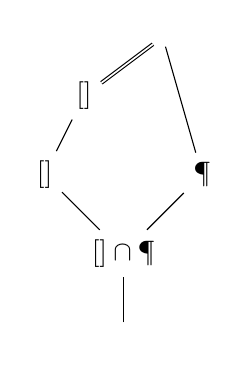
\begin{tikzpicture}
  \node at (0, 0) (nc) {$\NC$};
  \node at (0, 1) (both) {$\NNC[\polylog] \cap \P$};
  \node at (-1, 2) (nncpolylog) {$\NNC[\polylog]$};
  \node at (1, 2) (p) {$\P$};
  \node at (0.5, 3.75) (np) {$\NP$};
  \node at (-0.5, 3) (nnc) {$\NNC[\poly]$};

  \draw (nc) to (both);
  \draw (both) to (nncpolylog);
  \draw (both) to (p);
  \draw (p) to (np);
  \draw (nncpolylog) to (nnc);
  \draw[double] (nnc) to (np);
\end{tikzpicture}

\end{minipage}%
\begin{minipage}[t]{0.31\linewidth}
  \centering
  \begin{tikzpicture}
  \node at (0, 0) (nco) {$\NCO$};
  \node at (0, 1) (both) {$\ApxNCO \cap \PO$};
  \node at (-1, 2) (apxnco) {$\ApxNCO$};
  \node at (1, 2) (po) {$\PO$};
  \node at (0.5, 3.75) (npo) {$\NPO$};
  \node at (-0.5, 3) (nnco) {$\NNCO$};

  \draw (nco) to (both);
  \draw (both) to (apxnco);
  \draw (both) to (po);
  \draw (po) to (npo);
  \draw (apxnco) to (nnco);
  \draw[double] (nnco) -- (npo) node [rotate=45, midway] {\small$/$};
\end{tikzpicture}

\end{minipage}%
\begin{minipage}[t]{0.31\linewidth}
  \centering
  \begin{tikzpicture}
  \node at (0, 0) (fpnc) {$\para \NC$};
  \node at (0, 1) (both) {$\para \WNC[1] \cap \para \P$};
  \node at (-1, 2) (dontknow) {$\para \WNC[1]$};
  \node at (1, 2) (fpt) {$\para \P$};
  \node at (0.5, 3.75) (wp) {$\para \WP$};
  \node at (-0.5, 3) (wpp) {$\para \WNC$};

  \draw (fpnc) to (both);
  \draw (both) to (dontknow);
  \draw (both) to (fpt);
  \draw (fpt) to (wp);
  \draw (dontknow) to (wpp);
  \draw (wpp) to (wp);
\end{tikzpicture}

\end{minipage}

These inclusion diagrams shape how we approach all the problems in this paper.
Double lines represent equality, solid lines represent strict inequality under some reasonable complexity-theoretic assumptions, and dashed lines represent inclusions of unknown strictness or equality.
%% The fact that $\NNC[\poly] = \NP$ but $\NNCO \neq \NPO$ and $\para \WNC \neq \para \WP$ (under the assumption $\NC \neq \P$) leads us to conclude that viewing a computational problem as merely a decision problem is too coarse-grained an approach---it does not give enough information about the computational complexity of the problem.

%There is another view that we approach only indirectly in this work, the complexity of verification.
%% This is why $\NNCO$ differs from $\NPO$ and $\para \WNC$ differs from $\para \WP$: these classes take into account the complexity of verifying a solution.
%% The classes of decision problems $\NNC[\poly]$ and $\NP$ do not.

%% \todo{Descriptive complexity encompasses all of these; specifically for parallel complexity of optimization problems, see \autocite{kt93}.}

\section{TODO Make sure the introduction of each section covers these points}
We aim to show that there is a $\P$-complete problem that is also
\begin{enumerate}
\item[(D1)] not in $\NNC[\polylog]$ (\autoref{thm:pinpcp} provides one unless $P \subsetneq \polyL$),
\item[(D2)] in $\NNC[\polylog]$ but not in $\NC$ (unknown),
\item[(O1)] not in $\ApxNCO$ (\autocite[Theorem~3.25]{ncapproximation} provides one unless $\NC = \P$),
\item[(O2)] in $\ApxNCO$ but not in $\NCO$ (\autocite[Theorem~3.25]{ncapproximation} provides on unless $\NC = \P$),
\item[(P1)] not in $\para \WNC[1]$ (unknown),
\item[(P2)] in $\para \WNC[1]$ but not in $\para \NC$ (unknown).
\end{enumerate}
